\documentclass{aa}
\usepackage{preambule}
\usepackage[varg]{txfonts}

\def\l{\lambda}\def\L{\Lambda}

\begin{document}
\title{Redshift evolution of the SN stretch distribution}

%\subtitle{II. An example text with infinitesimal scientific value whose title
%and subtitle may also be split}

\author{N. Nicolas\inst{1}
    \and M. Rigault\inst{2}
}

%\offprints{R. Plemmons, \email{plemmons@...}}

\institute{Université de Lyon, F-69622, Lyon, France; Université de Lyon
    1, Villeurbanne; CNRS/IN2P3, Institut de Physique des Deux Infinis, Lyon
    \and Université Clermont Auvergne, CNRS/IN2P3, Laboratoire de
    Physique de Clermont, F-63000 Clermont-Ferrand, France.
}

\date{Received 2 November 1992 / Accepted 7 January 1993}

\abstract{Type Ia supernovae (SNe Ia) allow for the construction of the Hubble
    diagram, giving us information about the Universe's expansion and its
    fondamental components, one of which is dark energy. But systematic
    uncertainties are now starting to be limiting in our ability to measure
    those parameters. In particular, the physics of SNe Ia is still mostly
    unknown, and is thought not to change in time/with the redshift.}
    {In an attempt to reduce those uncertainties, we try to find an empirical
    law describing SNe Ia's length of explosion (stretch) evolution with the
redshift.}
    {We started by getting a complete sample representing all of the stretch
        distribution that Nature can give us, before using LsSFR measurments, an
        age tracer which evolution with redshift is known, that has been shown
        to have a strong correlation with the stretch. We compare their AICc, an
    estimator of the relative quality of statistical models that includes the
number of free parameters, to determine which ones describe besto the data.}
    {Models with an evolution of the stretch with the redshift have a better
    AICc than the ones without.}
    {We find that implementing these models allows us to fit the data better
    than models without stretch evolution.}

\keywords{Cosmology -- Type Ia Supernova -- Systematic uncertainties}
\maketitle

\section{Introduction}

Type Ia supernovae (SNe Ia) are now well-known for their capacity to determine
cosmological parameters: their study led to the discovery of the accelerated
expansion of the Universe (Riess 98, Perlmutter 99) through the name of "dark
energy", and they have been used continuously for better measurments since then
(Betoule 2014). They are acquired through their lightcurves, giving the
evolution of their luminosity from the time of explosion, in different
wavelength. 3 parameters are used to describe those: an amplitude, a width
(named "stretch") and a color (magnitude difference in the B and V bands).

The simple use of those is not enough for our aim, as SNe Ia have an intrinsec
dispersion of their luminosity of $\approx 0.4~mag$ that gives a huge
uncertainty on the determination of their distance modulus. Henceforth they are
standardized using the "brigther-slower" and "brighter-bluer" relations
(Philipps 93, Riess 96, Tripp 98) in the SALT2 algorithm (Guy 2007, 2010) that
fits the distance modulus which is expressed as
\begin{equation}
    \m = m_b + \a x_1 - \b c - M
\end{equation}
with $m_B$ the logarithm of their flux, $x_1$ their stretch, $c$ their color and
$M$ their intrinsec magnitude. This relation lowered their magnitude dispersion
to $\approx 0.15~mag$, allowing for previously mentioned accelerated
expansion to be discovered.

This Tripp estimator lies on the idea that this standardization doesn't change
with the redshift. However, Rigault 2015 showed that SNe Ia depend on their
environments, and these environments' properties evolve with the redshift. In
this Letter, we try to determine whether a stretch evolution with the redshift
allows for a better description of the collected data.

\section{Sample}\label{sec:sam}

We use data from 5 different surveys: Hubble Space Telescope (HST, REF),
Supernova Nearby Factory (SNf, REF), Supernova Legacy Survey (SNLS, Aster 2006,
Betoule 2014), Sloan DSS (SDSS, REF) and Panstarr-1 (PS1, REF). The last 3 had
selection effects that come from the "brighter-slower" and "brighter-bluer"
relations: the first SNe Ia that are missed by the instruments are the redder
and faster ones. That implies that taking all of these surveys' data would not
represent the stretch distribution that Nature could give us.

As such, we determined the maximum redshift at which we would cut these samples
to get complete ones. We used a statistical approach in lack of precise data
concerning the instruments' capacity to acquire fluxes. We proceeded by making
histograms of the surveys, and defining a function of the expected SNe Ia rate:
\begin{equation}
    N\St{SNe Ia} = a \times V\z
\end{equation}
with $a$ the density of SNe Ia and $V\z$ the volume of Universe in each bin.
Before selection effects, the histograms are supposed to grow proportionnaly to
$V\z$ assuming an homogeneous repartition of SNe Ia. When we start to miss some
supernovae, this growth is not followed anymore.

To determine this limit, we first took the observed counts in each bin of the
histograms. We then fitted $a$ on these counts for different numbers of bins
used to fit: the quality of the fit diminishes when we use bins that include
selection effects. To quantize this, we computed the expected counts from the
fitted $a$ in the same bins we used for the observed counts. That allowed us to
compute the poissonian probability in each bin, given by
\begin{equation}
    p(k) = \frac{\l^k}{k!}e^{-\l}
\end{equation}
with $k$ the expected counts, $\l$ the observed counts. This work is done 100
times with a random number of total bins, $a$ being fitted 10 times on a
different and random number of bins used to fit each time. We interpolate these
1000 poissonian evolutions to get one final result that is as close as possible
to accurately represent how the probability to follow the expected rate evolves.

To get the maximum redshift after which we stop following the expected rate, we
took the redshift for which we are at a 0.3 on the interpolated cumulative
distribution function. We chose that value to have a systematic analytical
result that matches what we expect from the histograms; its impact on the work
after is to be studied.

\begin{table}[htbp!]
    \centering
    \caption{Number of SNe Ia effectively used for each survey, totalling 689
    Sne Ia. TO CORRECT FOR NEW ZMAX}
    \label{tab:sample}
    \begin{tabularx}{\linewidth}{|Y*{1}{|Y}|}\hline
        \rowcolor{gray!15} Survey & Number of SNe Ia \\\hline\hline
        SNf & 141 \\\hline
        PS1 & 178 \\\hline
        SDSS & 206 \\\hline
        SNLS & 138 \\\hline
        HST & 26 \\\hline
    \end{tabularx}
\end{table}

\begin{figure}[htbp!]
    \centering
    \subfigure[Method]{\label{fig:zdet}
        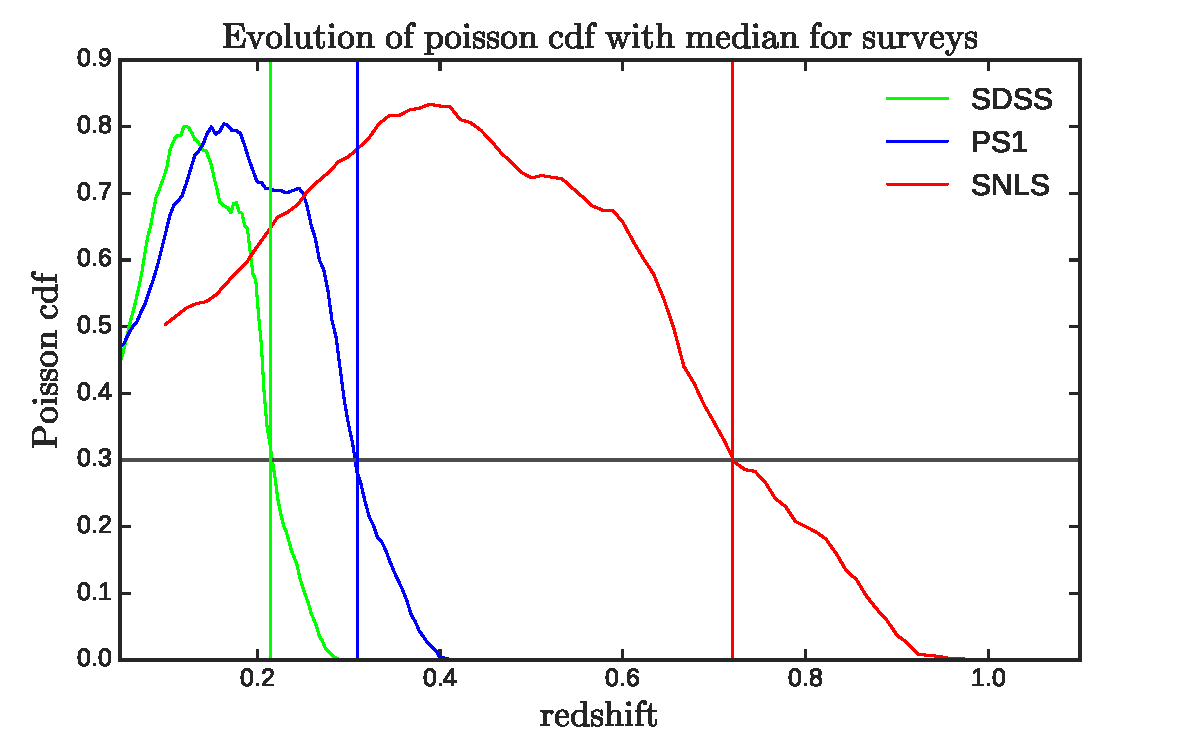
\includegraphics[width=\linewidth]{Article_figures/zmax_determination.pdf}}
    \subfigure[Result]{\label{fig:surveys_cuts}
    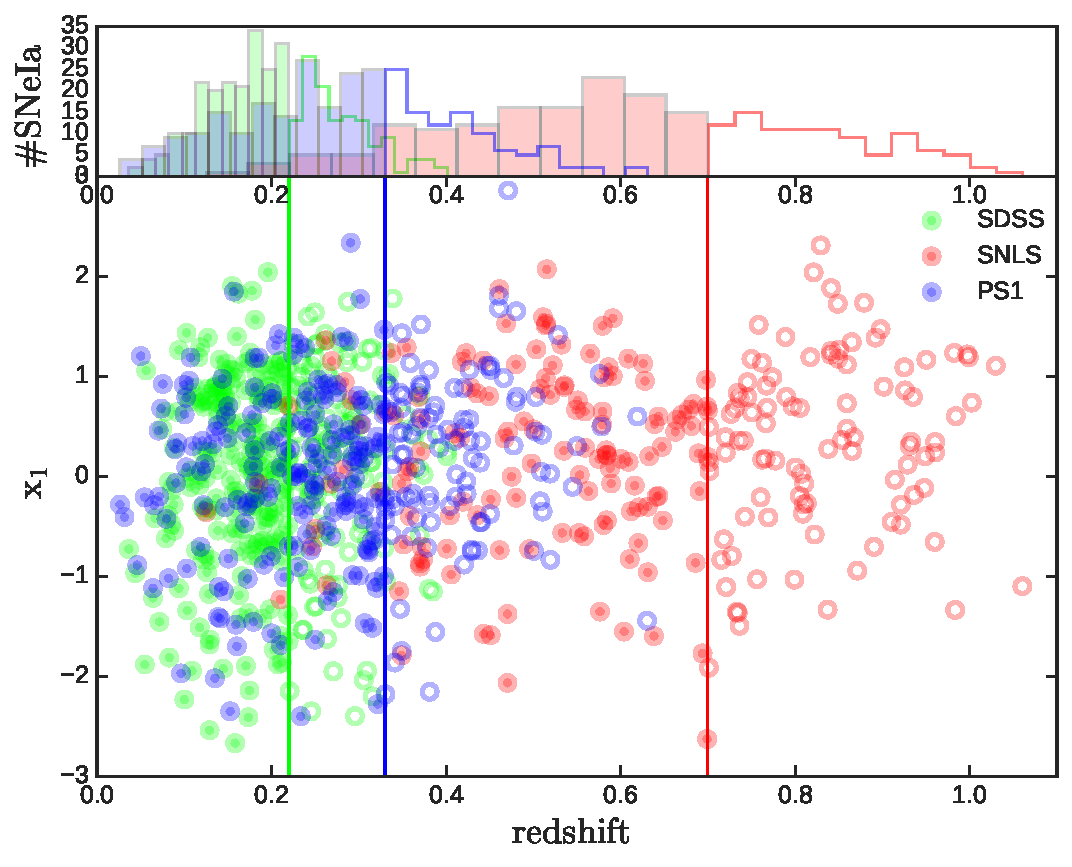
\includegraphics[width=\linewidth]{Article_figures/surveys_cuts_x.pdf}}
    \caption{(a) $z\St{max}$ determination from the interpolated poissonian
    evolutions; (b) SDSS, SNLS and PS1 samples cut at $z\St{max}$ as explained in
    section \ref{sec:sam}. The data we use is in plain markers.}
\end{figure}

\section{Method}

We used the LsSFR and stretch measurments from the SNf sample. The LsSFR has an
evolution with the redshift that is analytically known: calling $\de\z$ the
fraction of young stars and $\p\z$ the fraction of old ones, Rigault 2018 et +
find
\begin{equation}
    \frac{\de\z}{\p\z} \equiv \mathrm{LsSFR}\z = K\times \LF{1+z}^\f
\end{equation}
with $\f = 2.8$, and knowing $\de\z + \p\z = 1$:
\begin{align}
    \de\z & = \LF{K^{-1}\times \LF{1+z}^{-\f} +1}^{-1}\\
    \p\z & = \LF{K\times \LF{1+z}^{+\f} + 1}\um
\end{align}

\begin{figure}[htbp!]
    \centering
    \subfigure[Raw data]{\label{fig:snf_data}
        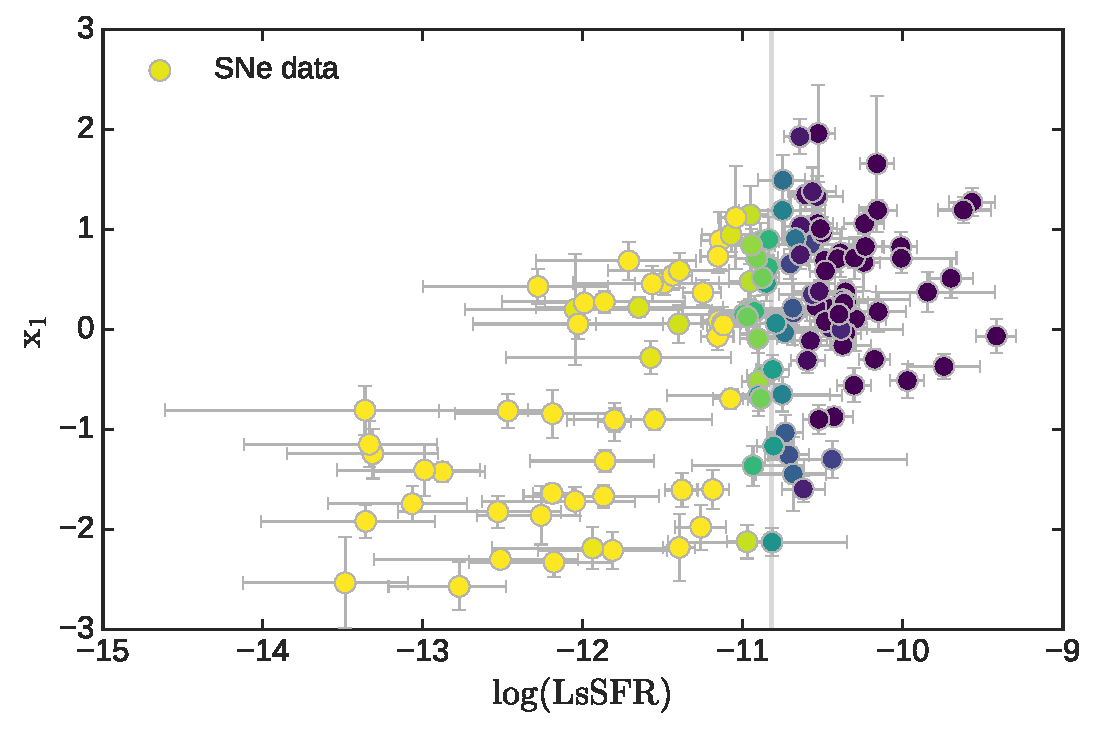
\includegraphics[width=\linewidth]{Article_figures/BiGaussian_onlydata.pdf}}
    \subfigure[First implemented model]{\label{fig:3G2M2SSNF}
        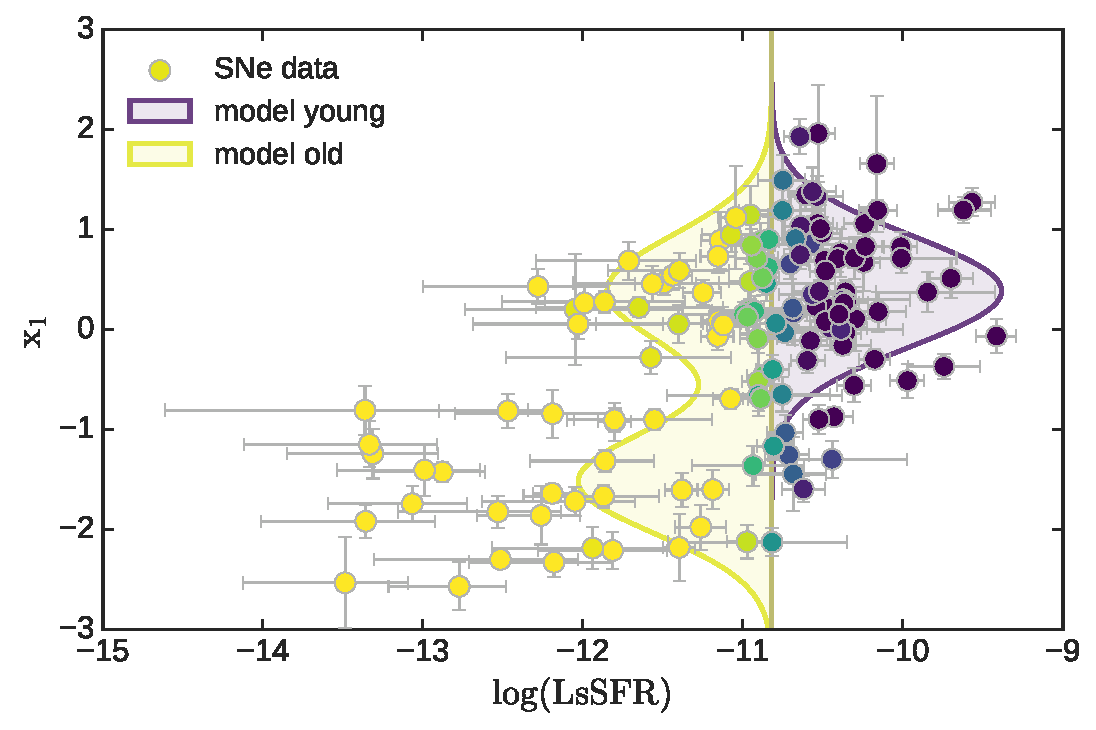
\includegraphics[width=\linewidth]{Article_figures/BiGaussian.pdf}}
    \caption{Stretch des supernovae étudiées par la collaboration SNF en
    fonction de log(LsSFR). La couleur représente la probabilité pour une
supernova d'être issue d'un jeune progéniteur.}
    \label{fig:mod_first}
\end{figure}

The goal is to find how the stretch depends on the LsSFR, distinguishing old and
young SNe which fractions evolve with the redshift, in order to have an
analytical law for the mean redshift evolution of the stretch. The measured data
on which we based our first model is plotted in figure \ref{fig:mod_first};
based of the shape of the $x_1$ vs LsSFR cloud, we implemented the following
model:
\begin{itemize}
    \item \textbf{young}: a gaussian of mean $\m_1$ and standard deviation
        $\s_1$, namely $\Nc_1 \equiv \Nc \LF{\m_1,\s_1}$;
    \item \textbf{old}: a linear combination between $\Nc_1$ and another
        gaussian $\Nc_2 \equiv \Nc \LF{\m_2,\s_2}$
\end{itemize}
As such, the probability to observe a young SNe Ia labeled "i" with a stretch
$x_1^i$ and error $\d x_1^i$ is
\begin{equation}
    p \LF{x_1^i, \d x_1{}^i|\m_1,\s_1} = \Nc \LF{\m_1, \Sq{\s_1{}^2 + \d
    x_1^i{}^2}}(x_1^i)
\end{equation}
and for an old one:
\begin{align}
    p(x_1^i, \d x_1^i | \m_{1,2}, \s_{1,2}, a) = a & \times \Nc \LF{\m_1,
    \sqrt{\s_1{}^2 + \d x_1^i{}^{2}}} (x_1^i) \ + \\ (1-a) & \times \Nc
    \LF{\m_2, \sqrt{ \s_2{}^2 + \d x_1^i{}^{2}}} (x_1^i), \nonumber 
\end{align}

\noindent where $a$ is the relative amplitude between the two gaussians.
Finally, the normalized stretch distribution at a given $z$ $\D\LF{x_1|z}$ is
the weigthed sum of both young and old stretch distributions given their
relative fraction $\de\z$:
\begin{equation}
    \D\LF{x_1|z} = \de\z\times\Nc_1 +
    \LF{1-\de\z} \times \LF{a\Nc_1 + (1-a)\Nc_2}
\end{equation}

We fitted it on SNf data, giving the results table \ref{tab:val}. For clarity
with the next models, we named it 3G2M2S$\St{SNf}$ for it has a total of 3
gaussians but with only 2 means and 2 standard deviations, and has been fitted
on SNf data only. 

We implemented and compared 10 models in total, 4 of which have an
evolution with the redshift from $\de\z$, and 6 don't ($\de\z = f =
\mathrm{cst}$). The ones with and evolution are:
\begin{itemize}
    \item 3G2M2S, the one we described (but fitted on all the data);
    \item 3G2M1S, where this time $\s_1 \equiv \s_2$;
    \item 2G2M2S, model taken from HOWELL 2009 where we added $\de\z$;
    \item 3G3M3S, with three independent gaussians.
\end{itemize}
The ones without a stretch evolution are the same ones but with an "F" implying
we set $\de\z = f = \mathrm{cst}$, and two others:
\begin{itemize}
    \item 1G1M1S, where there is no distinction between old and young SNe;
    \item 1G1M2S, taken from KESLLER 2017 and used in recent cosmological
        analysis SCOLNIC 2018. It's an asymetric model where
\end{itemize}

\begin{align}
 p(x_1^i, \d x_1^i | \m, \s_-, \s_+) = 
    \begin{cases}
        \mathcal{N} \LF{\m, \sqrt{\s_-{}^2 + \d x_1^i{}^{2}}} (x_1^i) & \text{if
        } x_1^i\geq \m\\
        \mathcal{N} \LF{\m, \sqrt{\s_+{}^2 + \d x_1^i{}^{2}}} (x_1^i), &
        \text{else}
    \end{cases}
\end{align} 

The fitted parameters are showed table \ref{tab:val}.

\begin{table}[htbp!]
    \centering
    \caption{Valeurs des paramètres pour différents modèles. En rouge les
    données aberrantes.}
    \label{tab:val}
    \begin{tabularx}{\linewidth}{|Y*{6}{|Y}|}\hline

        \rowcolor{gray!15} Modèle & $a$ & $f$ & $\m_1$ & $\s_1$ & $\m_2$ &
        $\s_2$ \\\hline\hline

        3G2M2S$_{\mathrm{SNf}}$ & $0.48 \pm 0.07$ & none & $0.39 \pm 0.07$ &
        $0.56 \pm 0.05$ & $-1.5 \pm 0.1$ & $0.52 \pm 0.09$ \\\hline

        3G2M2S & $0.48 \pm 0.17$ & none & $0.36 \pm 0.08$ & $0.61 \pm 0.05$ &
        $-1.3 \pm 0.2$ & $0.60 \pm 0.12$ \\\hline

        3G2M2SF & \textcolor{red}{$0.1 \pm 0.6$} & \textcolor{red}{$0.2 \pm
        0.6$} & $-0.9 \pm 0.7$ & $0.7 \pm 0.3$ & $0.5 \pm 0.2$ & $0.6 \pm 0.1$
        \\\hline

        3G2M1S & $0.47 \pm 0.07$ & none & $0.35 \pm 0.04$ & $0.61 \pm 0.03$ &
        $-1.25 \pm 0.10$ & $\s_1$ \\\hline

        3G2M1SF & \textcolor{red}{$0.2 \pm 0.9$} & $0.7 \pm 0.3$ & $0.36 \pm
        0.04$ & $0.60 \pm 0.03$ & $-1.23 \pm 0.10$ & $\s_1$ \\\hline

        2G2M2S & none & none & $0.49 \pm 0.04$ & $0.54 \pm 0.03$ & $-0.72 \pm
        0.08$ & $0.83 \pm 0.07$ \\\hline
        
        2G2M2SF & none & $0.3 \pm 0.2$ & $-0.9 \pm 0.6$ & $0.7 \pm 0.2$ & $0.5
        \pm 0.2$ & $0.56 \pm 0.09$ \\\hline

    \end{tabularx} \bigbreak

\begin{tabularx}{\linewidth}{|Y*{2}{|Y}|}\hline

    \rowcolor{gray!15} Modèle & $\m$ & $\s$ \\\hline\hline

    1G1M1S & $0.01 \pm 0.04$ & $0.90 \pm 0.03$ \\\hline

\end{tabularx} \bigbreak

\begin{tabularx}{\linewidth}{|Y*{3}{|Y}|}\hline

    \rowcolor{gray!15} Modèle & $\m$ & $\s_-$ & $\s_+$ \\\hline\hline

    1G1M2S & $0.16617 \pm 0.00004$ & $1.07 \pm 0.04$ & $0.69 \pm 0.03$ \\\hline

\end{tabularx} \bigbreak

\begin{tabularx}{\linewidth}{|Y*{8}{|Y}|}\hline

    \rowcolor{gray!15} Modèle & $a$ & $f$ & $\m_1$ & $\s_1$ & $\m_2$ & $\s_2$ &
    $m_3$ & $\s_3$ \\\hline\hline

    3G3M3S & $0.14 \pm 0.08$ & none & $0.51 \pm 0.06$ & $0.54 \pm 0.04$ & $-1.9
    \pm 0.2$ & $0.29 \pm 0.11$ & $-0.55 \pm 0.12$ & $0.67 \pm 0.15$ \\\hline
    
    3G3M3SF & $0.2 \pm 0.2 $ & $0.10 \pm 0.04 $ & $-1.7 \pm 0.2$ & $0.4 \pm 0.1$
            & $0.9 \pm 0.1$ & $0.3 \pm 0.2$ & $0.0 \pm 0.2$ & $0.7 \pm 0.1$
            \\\hline

\end{tabularx} \bigbreak

\end{table}



\section{Results}
To compare all these models, we use the Akaike Information Criterion corrected
for sample size (BURNHAM 2002), that penalises the increase of free parameters
in order to discourage overfitting:
\begin{equation}
    \mathrm{AICc} = \mathrm{AIC} + \LR{2k\LF{k+1}}{n - k - 1}
\end{equation}
with $\mathrm{AIC} = 2k - 2\ln\LF{\mathcal{L}}$, where $k$ is the number of free
parameters and $\Lc$ the likelihood. The probability for a model to be as
representative as the "best" one is given by:
\begin{equation}
    p(\mathrm{other} > \mathrm{best}) = \exp\LF{\D\mathrm{AICc}/2}
\end{equation}
As such, we obtain the results table \ref{tab:comp}.

\begin{table}[htbp!]
    \centering
    \caption{Comparaison des modèles. NR représente les modèles implémentés
             durant ce stage. (F) indique les modèles pour lesquels il n'y a pas
             d'évolution de la fraction de SNe~Ia jeunes et vieilles en fonction
             du redshift.}
    \label{tab:comp}
    \begin{tabularx}{\linewidth}{|Y*{6}{|Y}|}\hline

        \rowcolor{gray!15} Name & Description & Free param &
        $\ln\mathcal{L}$ & $AICc$ & $\D AICc$ & Proba \\\hline\hline

        3G2M1S & NR 1S & 4 & 1815 & 1823 & 0.0 & $1.0$ \\\hline

        3G2M2S & NR 2S & 5 & 1815  & 1825 & -2.0 & $3.6\times10^{-1}$ \\\hline

        2G2M2S & Howell & 4 & 1818  & 1826 & -3.4 & $1.8\times10^{-1}$ \\\hline

        3G3M3S & NR 3S & 7 & 1812  & 1826 & -3.6 & $1.6\times10^{-1}$ \\\hline

        3G3M3SF & NR 3S (F) & 8 & 1813 & 1829 & -6.3  & $4.3\times10^{-2}$
        \\\hline

        2G2M2SF & Howell (F) & 5 & 1823  & 1833 & -9.9 & $7.0\times10^{-3}$
        \\\hline

        3G2M1SF & NR 1S (F) & 5 & 1823  & 1833 & -10.4 & $5.5\times10^{-3}$
        \\\hline

        3G2M2SF & NR 2S (F) & 6 & 1823  & 1835 & -12.0 & $2.5\times10^{-3}$
        \\\hline

        1G1M2S & Kessler (F) & 3 & 1837  & 1843 & -20.2 & $4.1\times10^{-5}$
        \\\hline

        1G1M1S & 1 gauss. (F) & 2 & 1872 & 1876 & -53.5 &
        $2.4\times10^{-12}$\\\hline

    \end{tabularx}
\end{table}


We find that every model lacking an evolution of the stretch with the redshift
is systematically worse than those that implement it.

\section{Conclusion}
Stretch evolution with the redshift is a thing. Need to see if it has an impact
on the cosmology though.


\end{document}
